\chapter{Evaluation}

\section{Customer Requirements}

\subsection{Objective Evaluation}

\subsection{Simple and clear GUI}

\subsubsection{Having a very simple birds eye view image of the restaurant which is made out of shapes to ease the understanding of where each table is}
\begin{itemize}
	\item Objective has not been met
	\item I have used radio buttons instead to represent each table
\end{itemize}

\subsubsection{Label table with their corresponding number}
\begin{itemize}
	\item Objective has been met
	\item Each radio button is a representation of a table with the table number as the radio button label
\end{itemize}

\begin{figure}[H]
    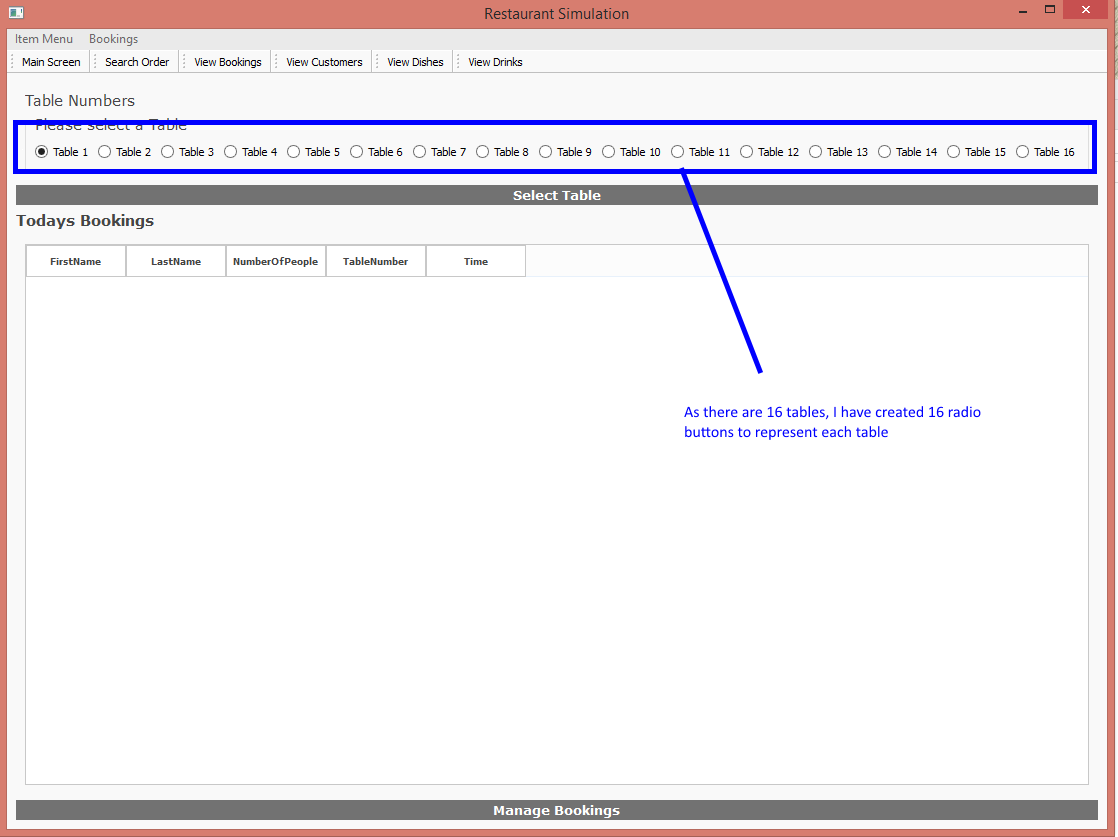
\includegraphics[width=\textwidth]{./Evaluation/images/radioButton}
    \caption{Main screen - highlighting the tables} \label{fig:radioButton}
\end{figure}

\subsubsection{Table shapes will be big so it won't be hard to click on them but not so big that 16 tables can fit on the GUI}
\begin{itemize}
	\item Objective has not been met
	\item I have used radio buttons to represent tables therefore I do not have any table shapes to meet this objective

\end{itemize}

\subsubsection{Clicking on table will bring up a window which shows the status such as the date and food items ordered with noticeable order modification options}
\begin{itemize} 
	\item Objective has mostly been met
	\item The user would have to select the table radio button and then click on Select Table
	\item The table has to be occupied to bring up the status window

\end{itemize}

\section{Effectiveness}

\subsection{Order alterations}
\subsubsection{Have clear Add, Delete and Create invoice buttons}
\begin{itemize}
	\item Objective has been met
	\item The application has clear Add and Delete buttons (User Questionnaire)
	\item The user can preview or print the invoice
\end{itemize}

\subsubsection{When the user chooses the add option, have an input box appear where the user can type in an ID for a dish/drink or the actual name of the dish/drink}
\begin{itemize}
	\item Objective has partially been met
	\item The current system only has the option to add an item by using the ID
\end{itemize}

\subsubsection{When the user chooses the add option, have an input box appear where the user can type in an ID for a dish/drink or the actual name of the dish/drink}
\begin{itemize}
	\item Objective has partially been met
	\item The current system only has the option to add an item by using the ID
\end{itemize}

\subsubsection{Make the input search function not case sensitive}
\begin{itemize}
	\item Objective has not been met
	\item There is no search function for the menu when adding an item to an order
\end{itemize}

\subsubsection{When user wants to delete a food item off the list, have clear red X boxes appear next to the name. When red X boxes are clicked on and with confirmation, the item gets deleted}
\begin{itemize}
	\item Objective has not been met
	\item I decided to not implement this feature in the system.
\end{itemize}

\subsubsection{ Have an up arrow or bottom arrow button just in case a customer orders another food item which is already on the list. The up arrow would increase the quantity of the item by 1 and the down arrow would decrease the item by 1 }
\begin{itemize}
	\item Objective has not been met
	\item I decided to not implement this feature in the system.
\end{itemize}

\subsubsection{ Clicking on create invoice button will clear the information on the table status and save the digital invoice in a folder}
\begin{itemize}
	\item Objective has not been met
	\item I created a "Finish" button to clear the information of the table so that the user can assign another customer to the table - this seemed more logical.
	\item I did not implement the 'save the digital invoice in a folder', instead, I made it an option to the user to print the invoice.
\end{itemize}

\subsection{Track Orders}

\subsubsection{ Drinks and dishes will be seperated by columns }
\begin{itemize}
	\item Objective has partially been met
	\item Drinks and dishes are seperated but by tables - clearer than using columns
\end{itemize}

\subsubsection{Clicking on a table will bring up a small window with the list of food items that the table has ordered, formatted like the invoice form shown on page 15. This also includes the date and table number.}
\begin{itemize}
	\item Objective has been met
	\item The user would have to select the table radio button and click on "Select Table" to track the order 
	\item As well as date and table number, I have included the time and number of people on the table.
\end{itemize}

\subsection{Invoice Creation}

\subsubsection{Automatically creating a digital invoice when a customer has finished}
\begin{itemize}
	\item bla
\end{itemize}

\subsubsection{Calculate total price}
\begin{itemize}
	\item Objective has been met
	\item (EVIDENCE)
\end{itemize}

\subsubsection{The digital invoice will look very similar to the invoice on page 15}
\begin{itemize}
	\item Objective has been met
	\item (EVIDENCE)
\end{itemize}

\subsubsection{Invoice will contain the items ordered, prices of each and total price}
\begin{itemize}
	\item Objective has been met
	\item (EVIDENCE)
\end{itemize}

\subsubsection{Have the option to print out invoice}
\begin{itemize}
	\item Objective has been met
	\item (EVIDENCE)
\end{itemize}

\subsection{Storing orders}

\subsubsection{When using the clear information button, the information is stored in the database}
\begin{itemize}
	\item Objective has not been met
	\item Information is stored automatically after the user has changed something on the order i.e added/deleted an item therefore there is no save process when pressing the clear information button( the "Finish" button)
\end{itemize}

\subsubsection{Filtering database for user if searching specific information}
\begin{itemize}
	\item Objective has not been met
	\item I have not implemented a filter feature
\end{itemize}

\subsubsection{Have an option to view database}
\begin{itemize}
	\item Objective has been met
	\item The tool bar is specifically designed to view the database
\end{itemize}
%include as many subsections as necessary for your objectives
\subsection{Objective Evaluation}

\section{Learnability}

\section{Usability}

\section{Maintainability}

\section{Suggestions for Improvement}

\section{End User Evidence}

\subsection{Questionnaires}

\subsection{Graphs}

\subsection{Written Statements}
